\section{Validation on industrial systems}
\label{sec:exp2}
The choice of the new system was a device under development for a \acs{WPMS}, which configuration is reported in Table \ref{tab:conf2}. This new optical bench was more robust than the previous one: the lasers were more thin and less noisy, while all the components are robustly fixed to the box. Nevertheless, it was dial by two different laser-camera pair. As we said in Chapter \ref{ch:sys_cmp}, it is primary to avoid occlusions when we take the profile of a train wheel, because of the presence of the flange. For this reasons, the target used for the second sets of experiments, was a section of a wheel (referred to as \textit{DIMA} in the following), shown in Figure \ref{fig:exp2-dima}. The measures of interests are reported in Table \ref{tab:exp2-measures}, all of them evaluable with a precision of $0.01 \, mm$. The abbreviations used are:
  \begin{itemize}
    \item \textit{FH} - Flange Height
    \item \textit{FT} - Flange Thickness
    \item \textit{QR} - qR quote 
    \item \textit{RW} - Rim Width
    \item \textit{RT} - Rim Thickness
  \end{itemize}

\begin{table}[h!]
  \centering
  \begin{tabular}{ccccc}
  \hline
  \multicolumn{5}{|c|}{\textbf{Camera}}                                                                                                                                                                            \\ \hline
  \multicolumn{1}{|c|}{\textbf{Name}} & \multicolumn{1}{c|}{\textbf{Size}}      & \multicolumn{1}{c|}{\textbf{Pixel size}} & \multicolumn{1}{c|}{\textbf{Lens Manufacturer}} & \multicolumn{1}{c|}{\textbf{Focal}} \\ \hline
  \multicolumn{1}{|l|}{}              & \multicolumn{1}{c|}{\textit{pix x pix}} & \multicolumn{1}{c|}{\textit{$\mu$m}}        & \multicolumn{1}{c|}{}                           & \multicolumn{1}{c|}{\textit{mm}}    \\ \hline
  \multicolumn{1}{|l|}{Arya}          & \multicolumn{1}{c|}{4096 x 3072}        & \multicolumn{1}{c|}{5.5}                 & \multicolumn{1}{c|}{Zeiss}                      & \multicolumn{1}{c|}{50}             \\ \hline
  \multicolumn{1}{l}{}                & \multicolumn{1}{l}{}                    & \multicolumn{1}{l}{}                     & \multicolumn{1}{l}{}                            & \multicolumn{1}{l}{}                \\ \cline{2-4}
  \multicolumn{1}{c|}{}               & \multicolumn{1}{c|}{\textbf{Laser}}     & \multicolumn{1}{c|}{}                    & \multicolumn{1}{c|}{}                           &                                     \\ \cline{2-4}
  \multicolumn{1}{c|}{}               & \multicolumn{1}{c|}{\textbf{Frequency}} & \multicolumn{1}{c|}{\textbf{Power}}      & \multicolumn{1}{c|}{\textbf{Aperture}}          &                                     \\ \cline{2-4}
  \multicolumn{1}{c|}{\textit{}}      & \multicolumn{1}{c|}{\textit{nm}}        & \multicolumn{1}{c|}{\textit{W}}          & \multicolumn{1}{c|}{\textit{degree}}            & \textit{}                           \\ \cline{2-4}
  \multicolumn{1}{c|}{}               & \multicolumn{1}{c|}{450}                & \multicolumn{1}{c|}{3.5}                 & \multicolumn{1}{c|}{45}                         &                                     \\ \cline{2-4}
  \end{tabular}
  
  \caption{Configuration of the second system.}
  \label{tab:conf2}
\end{table}

The first step was to compare the results of our calibration algorithm with the ones of the company. Differently from the previous case, the presence of two laser-camera pair required to calibrate both of them, independently one from the other. After that, a second round of calibration was needed to determine the relations to use to merge the two profiles. Note that this scenario gave us some issue later, in particular because of the two pairs
  \begin{figure}
    \centering
    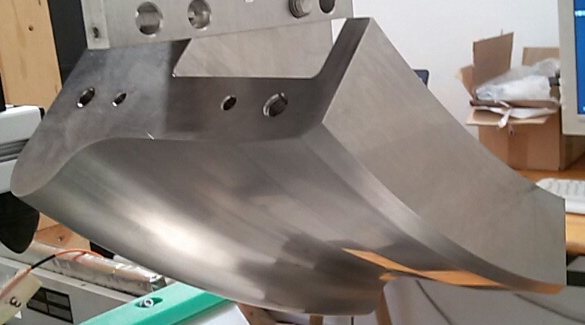
\includegraphics[width=\textwidth]{./images/analysis/exp2/DIMA.jpg}
    \caption{Photo of the DIMA}
    \label{fig:exp2-dima}
  \end{figure}
\vfill
  \begin{table}
\centering
\begin{tabular}{|c|c|c|c|c|}
\hline
\textbf{FH}   & \textbf{FT}   & \textbf{QR}   & \textbf{RW}   & \textbf{RT}   \\ \hline
\textit{(mm)} & \textit{(mm)} & \textit{(mm)} & \textit{(mm)} & \textit{(mm)} \\ \hline
$28.00$       & $32.52$       & $10.81$       & $135.01$      & $47.11$         \\ \hline
\end{tabular}
\caption{Measures of the DIMA}
\label{tab:exp2-measures}
\end{table}
\vfill
  \begin{figure}
    \centering
    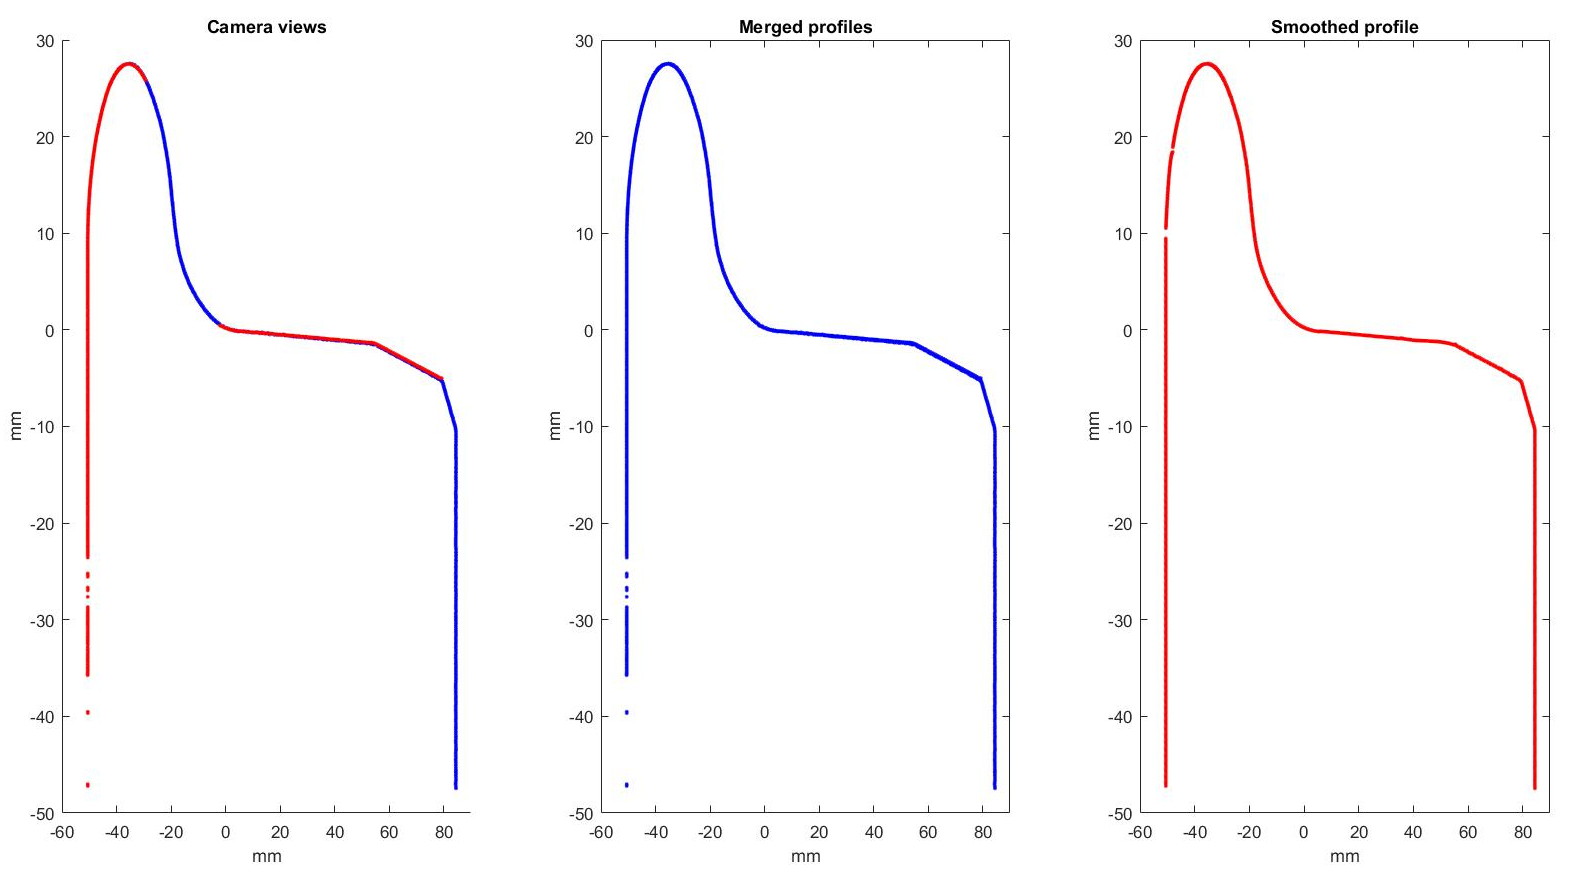
\includegraphics[width=\textwidth]{./images/analysis/exp2/wheel_steps.jpg}
    \caption{Steps used to merged the two profiles}
    \label{fig:exp2-merged}
  \end{figure}
\noindent
which used two different configurations, e.g. in terms of baselines length and triangulation angles. However, once again, all the parameters where comparable between the two algorithms, thus we continued with our analysis.

The second step, was the evaluation of the profile. Using the results of the previous set of experiments, we focused only on the \textit{center of mass}, \textit{Blais\&Rioux} and \textit{FIR} filters, ignoring the others. The windows used where of $16$ and $20$ pixels for each filter. After several attempts we correctly merged the two profiles collected by the two laser-camera pairs. To do that, we first converted the filtered laser in the world reference system, than we superimposed the two profiles and merged them in the same data structure. At the end we smoothed a bit the obtained profile, in order to reduce the effect of noise and the laser thickness, especially along the inner ad outer sides. The result reached is shown in Figure \ref{fig:exp2-merged}. \\

As shown in the last sub-plot, we had to pay attention when using \textsc{MatLab} functions: to increase the precision of this process, we decided to split the wheel's section in many parts, using the keypoints described above as extreme points of these curves; thus, we used a different mathematical model to smooth each part. During this process, it could happen that some gaps appear in the smoothed profile, reducing the precision of points location. As we will see, we can consider these errors negligible in our working conditions. \\

Finally, numerical results are shown. In Table \ref{tab:exp2:refereces} we reported an approximation of the errors committed at the center of the \acs{FOV}. It is already possible to see that, despite the improving given by the filters at pixel level, we haven't a same increase on the world reference system, i.e. in $mm$. Carefully analysing each step of the model, we noticed that the performance decreased on Equation \ref{eq:model:err:disc} and on Equation \ref{eq:det_a}. In the first case it is simple to understand why: the multiplication by the pixel size considerably reduces the weight of the error, especially if the pixel size is in the order of tenths of a millimiter. To be precise, this is not an error reduction, rather a change of scale, from pixel to millimeters; the smaller the pixel is, the smaller is the weight of the error. Regarding the second case, instead, we didn't find a good answer that can explain what happened. From our point of view, we could interpret this situation as an another change of reference system, from the camera to the world. However, the change of unit of measure was performed in case before. The only thing that can help us is that, a variation in the point in the space corresponds to a much smaller variation in the sensor, so the error is more apparent on the latter plane, rather than in the world.
  \begin{table}[h!]
  \centering
  \begin{tabular}{|l|r|r|r|r|}
    \hline
    \multirow{2}{*}{}  & \multicolumn{1}{c|}{\textbf{Approximation}} & \multicolumn{1}{c|}{\textbf{Y}}    & \multicolumn{1}{c|}{\textbf{X}}    & \multicolumn{1}{c|}{\textbf{Point error}} \\
	\hline
                       & \multicolumn{1}{c|}{\textit{(pixel)}}    & \multicolumn{1}{c|}{\textit{(mm)}} & \multicolumn{1}{c|}{\textit{(mm)}} & \multicolumn{1}{c|}{\textit{(mm)}}  \\
	\hline
    \textbf{Pixel}    & 0,4083    & 0,0353    & 0,0199    & 0,0405 \\
    \hline
    \textbf{CoM 16}   & 0,1877    & 0,0322    & 0,0195    & 0,0377 \\
    \hline
    \textbf{CoM 20}   & 0,1062    & 0,0316    & 0,0195    & 0,0372 \\
    \hline
    \textbf{BR 16}    & 0,1413    & 0,0319    & 0,0195    & 0,0374 \\
    \hline
    \textbf{BR 20}    & 0,1302    & 0,0318    & 0,0195    & 0,0373 \\
    \hline
    \textbf{FIR}      & 0,2587    & 0,0330    & 0,0196    & 0,0384 \\
    \hline
  \end{tabular}
  
  \caption{Reference values for propagation of the error (model output at the center of the \acs{FOV})}
  \label{tab:exp2:refereces}
\end{table}

Nevertheless, a comparison from theoretical and real results is shown in Table \ref{tab:exp2:means}. The values are the averages over the five measures mentioned above, evaluated using the points shown in Figure \ref{fig:exp2-cad}. As of the theoretical measures, they are estimated as differences between the values in column \textit{point error} of the Table \ref{tab:exp2:refereces}, but evaluated for the keypoints in figure. As we can see, the model is validated: the variation between theoretical and empirical results is comparable with the theoretical variance, so we can consider the results identical. There are only few consideration to take into account.
  \begin{table}[t!]
  \centering
  \begin{tabular}{|l|rr|rr|}
  \hline
  \multirow{3}{*}{} & \multicolumn{1}{c}{\textbf{\begin{tabular}[c]{@{}c@{}}Theoretical\\ Errors\end{tabular}}} & \multicolumn{1}{c|}{\textbf{Variance}} & \multicolumn{1}{c}{\textbf{\begin{tabular}[c]{@{}c@{}}Empirical\\ Errors\end{tabular}}} & \multicolumn{1}{c|}{\textbf{Variance}} \\
  \hline
  & \multicolumn{1}{c}{\textit{$(\mu m)$}}    & \multicolumn{1}{c|}{\textit{$(\mu m)$}}     & \multicolumn{1}{c}{\textit{$(\mu m)$}}    & \multicolumn{1}{c|}{\textit{$(\mu m)$}}     \\
  \hline
  \textbf{Pixel}     & 36.2    & 0.001400    & 105.1    & 5.9 \\
  \hline
  \textbf{CoM 16}    & 29.6    & 0.000973    & 32.1     & 0.5 \\
  \hline
  \textbf{CoM 20}    & 28.2    & 0.000823    & 33.5     & 0.7 \\
  \hline
  \textbf{BR 16}     & 28.8    & 0.000917    & 32.8     & 0.6 \\
  \hline
  \textbf{BR 20}     & 28.6    & 0.000875    & 30.0     & 0.4 \\
  \hline
  \textbf{FIR}       & 31.4    & 0.001240    & 29.6     & 0.3 \\
  \hline
  \end{tabular}
  
  \caption{Averages of the computed measures}
  \label{tab:exp2:means}
\end{table}

  \begin{figure}[t!]
    \centering
    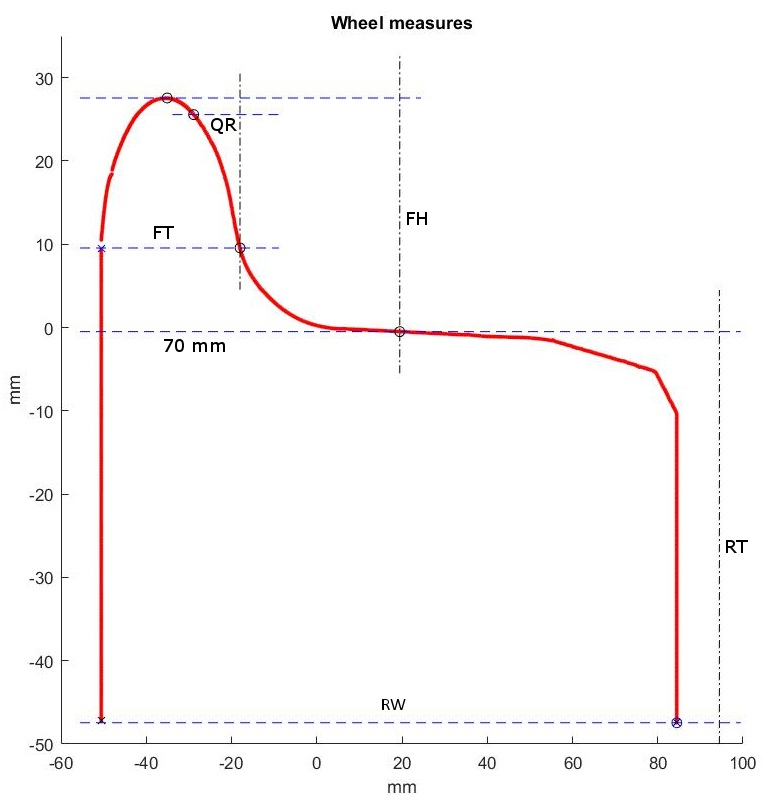
\includegraphics[width=0.88\textwidth]{./images/analysis/exp2/wheel_profile_mod.jpg}
    \caption{Analysed profile, with measure indication, CAD style.}
    \label{fig:exp2-cad}
  \end{figure}
As we said at the beginning of this section, we are using two laser-camera pairs, which results are merged to obtain the profile. The two systems used different configurations, in particular different triangulation angles and baselines. Despite this, differences are very small in terms of absolute values, we noticed that they lead to different output models, i.e. different error approximations. In Table \ref{tab:exp2:refereces}, as in the other phases of our analysis, the values in columns \textit{Y} and \textit{X} are the means of the two models. In this case we consider the means, instead of the error propagation for the variance in Equation \ref{eq:exp:var-prop}, because we didn't know to which piece of the profile the selected point belongs. Statistically, we had a probability of an half, thus we considered the mean as the most appropriate operator.

Another doubt we still had, regards the tuning of the model. Also in this case, we missed some informations, such as the precision of the Scheimpflug angle, or the orientation of the laser (it is a degree of freedom of the system). Thus, we needed to perform a tuning in order to balance the output with the empirical results. Notwithstanding the values used were reasonable with respect to the system structure, we thought that in this way, we mixed some errors due to the model and to the algorithm used to align and merge the two profiles. \\

To conclude, we can say that the model seems to be correct. This last set of tests allowed to underline the fact that it is a good approximation of the real scenarios, however, it has some degrees of freedom that must be analysed to get reasonable results. Also in this case, we remarked the importance of using windows comparable to the laser width, on the contrary the effects noise present in the acquired frames could be great enough to predominate on the laser. As far as the camera is concerned, we used here a sensor with pixels sizes smaller than the camera used in the previous section. As we can see, reducing pixels size reduces considerably the performances of the sub-pixel filters: this is reasonable if we think that a smaller pixel represents a smaller part of the world. \\
Two more considerations before continuing, concerning the resolution of the camera and the effects of noise in the frame. During our analysis we noticed that the empirical errors we obtained were very similar to the nominal resolution of the camera. This observation suggested us to control if a same thing happened in the previous set of experiments, and we noticed that it was quite true. Looking at the noise, however, we have noticed how to change the preprocessing of the image being analysed, changing the values of the empirical errors. More in-depth analyses are discussed in the sections bellow.
%